\documentclass{standalone}
\usepackage{tikz}
\usetikzlibrary{patterns, positioning}


\begin{document}
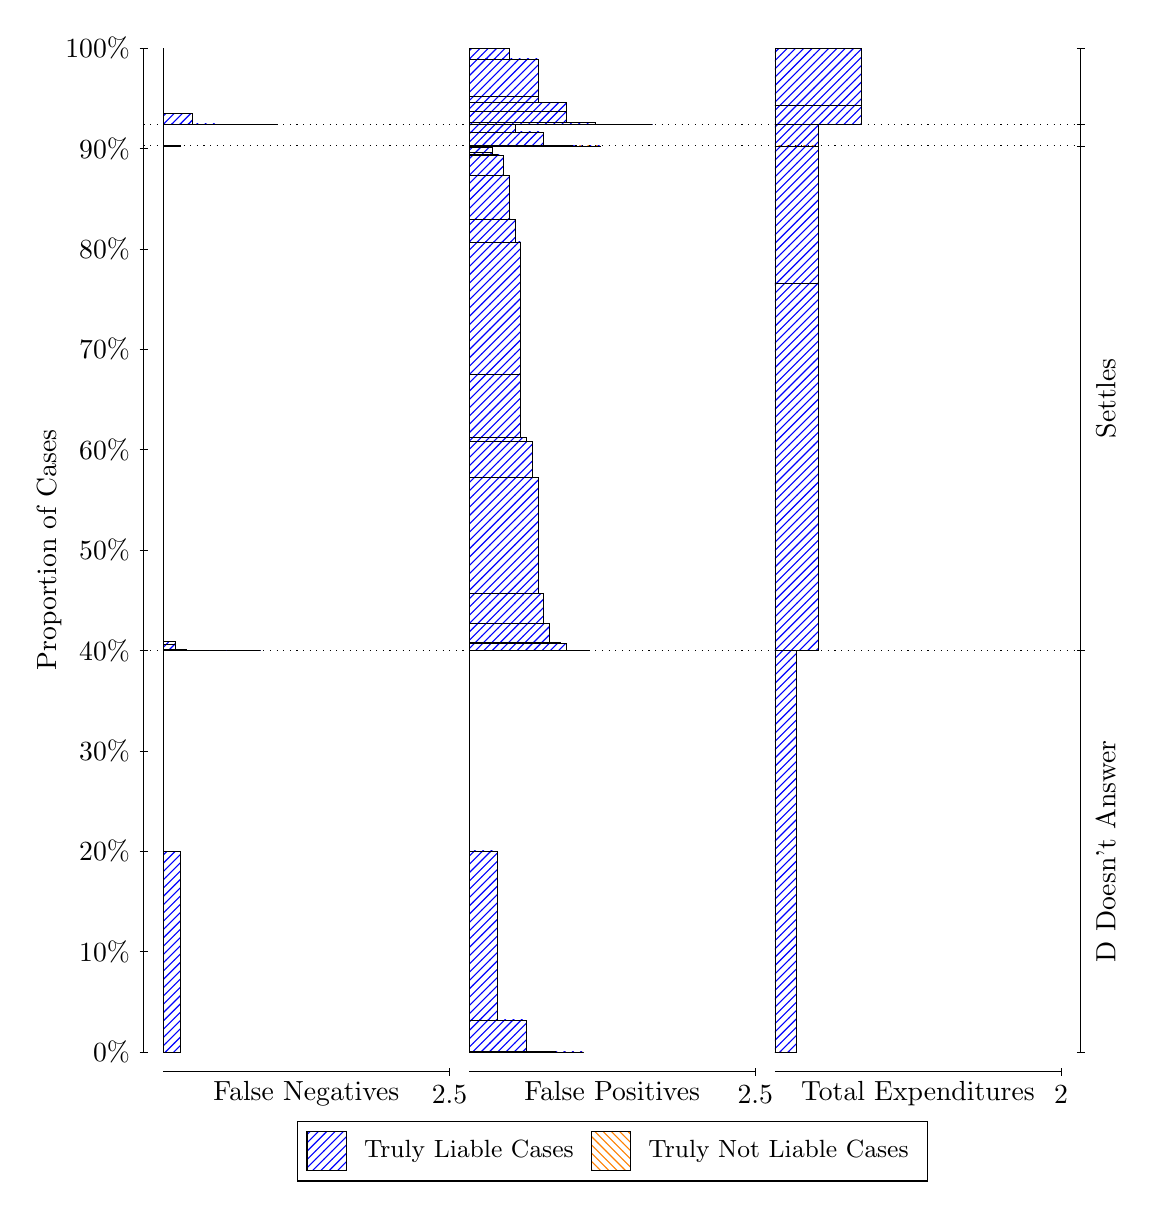
\begin{tikzpicture}
\draw[black, very thin] (1.5,1.75) -- (1.5,14.5);
\node[rotate=90, text=black, anchor=center] at (0.3, 8.125) {Proportion of Cases};
\draw[black, very thin] (1.45,1.75) -- (1.55,1.75);
\node[text=black, anchor=east] at (1.45, 1.75) {0\%};
\draw[black, very thin] (1.45,3.025) -- (1.55,3.025);
\node[text=black, anchor=east] at (1.45, 3.025) {10\%};
\draw[black, very thin] (1.45,4.3) -- (1.55,4.3);
\node[text=black, anchor=east] at (1.45, 4.3) {20\%};
\draw[black, very thin] (1.45,5.575) -- (1.55,5.575);
\node[text=black, anchor=east] at (1.45, 5.575) {30\%};
\draw[black, very thin] (1.45,6.85) -- (1.55,6.85);
\node[text=black, anchor=east] at (1.45, 6.85) {40\%};
\draw[black, very thin] (1.45,8.125) -- (1.55,8.125);
\node[text=black, anchor=east] at (1.45, 8.125) {50\%};
\draw[black, very thin] (1.45,9.4) -- (1.55,9.4);
\node[text=black, anchor=east] at (1.45, 9.4) {60\%};
\draw[black, very thin] (1.45,10.675) -- (1.55,10.675);
\node[text=black, anchor=east] at (1.45, 10.675) {70\%};
\draw[black, very thin] (1.45,11.95) -- (1.55,11.95);
\node[text=black, anchor=east] at (1.45, 11.95) {80\%};
\draw[black, very thin] (1.45,13.225) -- (1.55,13.225);
\node[text=black, anchor=east] at (1.45, 13.225) {90\%};
\draw[black, very thin] (1.45,14.5) -- (1.55,14.5);
\node[text=black, anchor=east] at (1.45, 14.5) {100\%};

\draw[black, very thin] (13.4,1.75) -- (13.4,14.5);
\draw[black, very thin] (13.35,1.75) -- (13.45,1.75);
\node[anchor=west] at (13.35, 1.75) {};
\draw[black, very thin] (13.35,6.8488) -- (13.45,6.8488);
\node[anchor=west] at (13.35, 6.8488) {};
\draw[black, very thin] (13.35,13.257) -- (13.45,13.257);
\node[anchor=west] at (13.35, 13.257) {};
\draw[black, very thin] (13.35,13.533) -- (13.45,13.533);
\node[anchor=west] at (13.35, 13.533) {};
\draw[black, very thin] (13.35,14.5) -- (13.45,14.5);
\node[anchor=west] at (13.35, 14.5) {};

\draw[black, very thin, pattern color=blue, pattern=north east lines] (1.75,1.75) rectangle (1.968,4.2958);
\draw[black, very thin, pattern color=orange, pattern=north west lines] (1.75,4.2958) rectangle (1.75,4.2958);
\draw[black, very thin, pattern color=blue, pattern=north east lines] (1.75,4.2958) rectangle (1.75,6.8488);
\draw[black, very thin, pattern color=blue, pattern=north east lines] (1.75,6.8488) rectangle (2.9853,6.8488);
\draw[black, very thin, pattern color=blue, pattern=north east lines] (1.75,6.8488) rectangle (2.6947,6.8488);
\draw[black, very thin, pattern color=blue, pattern=north east lines] (1.75,6.8488) rectangle (2.622,6.8488);
\draw[black, very thin, pattern color=blue, pattern=north east lines] (1.75,6.8488) rectangle (2.5493,6.8488);
\draw[black, very thin, pattern color=blue, pattern=north east lines] (1.75,6.8488) rectangle (2.404,6.8488);
\draw[black, very thin, pattern color=blue, pattern=north east lines] (1.75,6.8488) rectangle (2.3313,6.8488);
\draw[black, very thin, pattern color=blue, pattern=north east lines] (1.75,6.8488) rectangle (2.2587,6.8488);
\draw[black, very thin, pattern color=blue, pattern=north east lines] (1.75,6.8488) rectangle (2.186,6.8488);
\draw[black, very thin, pattern color=blue, pattern=north east lines] (1.75,6.8488) rectangle (2.1133,6.8518);
\draw[black, very thin, pattern color=blue, pattern=north east lines] (1.75,6.8518) rectangle (2.0407,6.8643);
\draw[black, very thin, pattern color=blue, pattern=north east lines] (1.75,6.8643) rectangle (1.968,6.8655);
\draw[black, very thin, pattern color=blue, pattern=north east lines] (1.75,6.8655) rectangle (1.8953,6.9288);
\draw[black, very thin, pattern color=blue, pattern=north east lines] (1.75,6.9288) rectangle (1.8953,6.9613);
\draw[black, very thin, pattern color=blue, pattern=north east lines] (1.75,6.9613) rectangle (1.8227,6.963);
\draw[black, very thin, pattern color=orange, pattern=north west lines] (1.75,6.963) rectangle (1.75,6.963);
\draw[black, very thin, pattern color=blue, pattern=north east lines] (1.75,6.963) rectangle (1.75,13.257);
\draw[black, very thin, pattern color=blue, pattern=north east lines] (1.75,13.257) rectangle (1.968,13.259);
\draw[black, very thin, pattern color=orange, pattern=north west lines] (1.75,13.259) rectangle (1.75,13.259);
\draw[black, very thin, pattern color=blue, pattern=north east lines] (1.75,13.259) rectangle (1.75,13.533);
\draw[black, very thin, pattern color=blue, pattern=north east lines] (1.75,13.533) rectangle (3.2033,13.533);
\draw[black, very thin, pattern color=blue, pattern=north east lines] (1.75,13.533) rectangle (2.84,13.533);
\draw[black, very thin, pattern color=blue, pattern=north east lines] (1.75,13.533) rectangle (2.4767,13.537);
\draw[black, very thin, pattern color=blue, pattern=north east lines] (1.75,13.537) rectangle (2.1133,13.671);
\draw[black, very thin, pattern color=orange, pattern=north west lines] (1.75,13.671) rectangle (1.75,13.671);
\draw[black, very thin, pattern color=blue, pattern=north east lines] (1.75,13.671) rectangle (1.75,14.5);
\draw[black, very thin, pattern color=orange, pattern=north west lines] (5.6333,1.75) rectangle (7.0867,1.75);
\draw[black, very thin, pattern color=blue, pattern=north east lines] (5.6333,1.75) rectangle (7.0867,1.75);
\draw[black, very thin, pattern color=blue, pattern=north east lines] (5.6333,1.75) rectangle (6.7233,1.7535);
\draw[black, very thin, pattern color=blue, pattern=north east lines] (5.6333,1.7535) rectangle (6.36,2.158);
\draw[black, very thin, pattern color=blue, pattern=north east lines] (5.6333,2.158) rectangle (5.9967,4.303);
\draw[black, very thin, pattern color=blue, pattern=north east lines] (5.6333,4.303) rectangle (5.6333,6.8488);
\draw[black, very thin, pattern color=orange, pattern=north west lines] (5.6333,6.8488) rectangle (7.1593,6.8488);
\draw[black, very thin, pattern color=blue, pattern=north east lines] (5.6333,6.8488) rectangle (7.1593,6.8488);
\draw[black, very thin, pattern color=orange, pattern=north west lines] (5.6333,6.8488) rectangle (7.014,6.8488);
\draw[black, very thin, pattern color=blue, pattern=north east lines] (5.6333,6.8488) rectangle (7.014,6.8493);
\draw[black, very thin, pattern color=orange, pattern=north west lines] (5.6333,6.8493) rectangle (6.8687,6.8493);
\draw[black, very thin, pattern color=blue, pattern=north east lines] (5.6333,6.8493) rectangle (6.8687,6.9392);
\draw[black, very thin, pattern color=blue, pattern=north east lines] (5.6333,6.9392) rectangle (6.796,6.9535);
\draw[black, very thin, pattern color=orange, pattern=north west lines] (5.6333,6.9535) rectangle (6.7233,6.9535);
\draw[black, very thin, pattern color=blue, pattern=north east lines] (5.6333,6.9535) rectangle (6.7233,6.9559);
\draw[black, very thin, pattern color=blue, pattern=north east lines] (5.6333,6.9559) rectangle (6.6507,7.1881);
\draw[black, very thin, pattern color=orange, pattern=north west lines] (5.6333,7.1881) rectangle (6.578,7.1881);
\draw[black, very thin, pattern color=blue, pattern=north east lines] (5.6333,7.1881) rectangle (6.578,7.5759);
\draw[black, very thin, pattern color=blue, pattern=north east lines] (5.6333,7.5759) rectangle (6.5053,9.046);
\draw[black, very thin, pattern color=blue, pattern=north east lines] (5.6333,9.046) rectangle (6.4327,9.5081);
\draw[black, very thin, pattern color=blue, pattern=north east lines] (5.6333,9.5081) rectangle (6.36,9.5542);
\draw[black, very thin, pattern color=blue, pattern=north east lines] (5.6333,9.5542) rectangle (6.2873,10.358);
\draw[black, very thin, pattern color=orange, pattern=north west lines] (5.6333,10.358) rectangle (6.2873,10.358);
\draw[black, very thin, pattern color=blue, pattern=north east lines] (5.6333,10.358) rectangle (6.2873,12.037);
\draw[black, very thin, pattern color=blue, pattern=north east lines] (5.6333,12.037) rectangle (6.2147,12.329);
\draw[black, very thin, pattern color=blue, pattern=north east lines] (5.6333,12.329) rectangle (6.142,12.883);
\draw[black, very thin, pattern color=blue, pattern=north east lines] (5.6333,12.883) rectangle (6.0693,13.143);
\draw[black, very thin, pattern color=blue, pattern=north east lines] (5.6333,13.143) rectangle (5.9967,13.145);
\draw[black, very thin, pattern color=blue, pattern=north east lines] (5.6333,13.145) rectangle (5.924,13.178);
\draw[black, very thin, pattern color=blue, pattern=north east lines] (5.6333,13.178) rectangle (5.924,13.241);
\draw[black, very thin, pattern color=blue, pattern=north east lines] (5.6333,13.241) rectangle (5.8513,13.242);
\draw[black, very thin, pattern color=blue, pattern=north east lines] (5.6333,13.242) rectangle (5.7787,13.255);
\draw[black, very thin, pattern color=blue, pattern=north east lines] (5.6333,13.255) rectangle (5.706,13.257);
\draw[black, very thin, pattern color=blue, pattern=north east lines] (5.6333,13.257) rectangle (5.6333,13.257);
\draw[black, very thin, pattern color=orange, pattern=north west lines] (5.6333,13.257) rectangle (7.3047,13.257);
\draw[black, very thin, pattern color=blue, pattern=north east lines] (5.6333,13.257) rectangle (7.3047,13.257);
\draw[black, very thin, pattern color=blue, pattern=north east lines] (5.6333,13.257) rectangle (6.9413,13.263);
\draw[black, very thin, pattern color=blue, pattern=north east lines] (5.6333,13.263) rectangle (6.578,13.435);
\draw[black, very thin, pattern color=blue, pattern=north east lines] (5.6333,13.435) rectangle (6.2147,13.532);
\draw[black, very thin, pattern color=blue, pattern=north east lines] (5.6333,13.532) rectangle (5.8513,13.533);
\draw[black, very thin, pattern color=orange, pattern=north west lines] (5.6333,13.533) rectangle (7.9587,13.533);
\draw[black, very thin, pattern color=blue, pattern=north east lines] (5.6333,13.533) rectangle (7.9587,13.533);
\draw[black, very thin, pattern color=orange, pattern=north west lines] (5.6333,13.533) rectangle (7.5953,13.533);
\draw[black, very thin, pattern color=blue, pattern=north east lines] (5.6333,13.533) rectangle (7.5953,13.534);
\draw[black, very thin, pattern color=orange, pattern=north west lines] (5.6333,13.534) rectangle (7.232,13.534);
\draw[black, very thin, pattern color=blue, pattern=north east lines] (5.6333,13.534) rectangle (7.232,13.558);
\draw[black, very thin, pattern color=blue, pattern=north east lines] (5.6333,13.558) rectangle (6.8687,13.693);
\draw[black, very thin, pattern color=orange, pattern=north west lines] (5.6333,13.693) rectangle (6.8687,13.693);
\draw[black, very thin, pattern color=blue, pattern=north east lines] (5.6333,13.693) rectangle (6.8687,13.813);
\draw[black, very thin, pattern color=blue, pattern=north east lines] (5.6333,13.813) rectangle (6.5053,13.889);
\draw[black, very thin, pattern color=orange, pattern=north west lines] (5.6333,13.889) rectangle (6.5053,13.889);
\draw[black, very thin, pattern color=blue, pattern=north east lines] (5.6333,13.889) rectangle (6.5053,14.362);
\draw[black, very thin, pattern color=blue, pattern=north east lines] (5.6333,14.362) rectangle (6.142,14.363);
\draw[black, very thin, pattern color=blue, pattern=north east lines] (5.6333,14.363) rectangle (6.142,14.497);
\draw[black, very thin, pattern color=blue, pattern=north east lines] (5.6333,14.497) rectangle (5.7787,14.497);
\draw[black, very thin, pattern color=blue, pattern=north east lines] (5.6333,14.497) rectangle (5.7787,14.5);
\draw[black, very thin, pattern color=blue, pattern=north east lines] (5.6333,14.5) rectangle (5.6333,14.5);
\draw[black, very thin, pattern color=orange, pattern=north west lines] (9.5167,1.75) rectangle (9.7892,1.75);
\draw[black, very thin, pattern color=blue, pattern=north east lines] (9.5167,1.75) rectangle (9.7892,6.8488);
\draw[black, very thin, pattern color=orange, pattern=north west lines] (9.5167,6.8488) rectangle (10.062,6.8488);
\draw[black, very thin, pattern color=blue, pattern=north east lines] (9.5167,6.8488) rectangle (10.062,11.515);
\draw[black, very thin, pattern color=orange, pattern=north west lines] (9.5167,11.515) rectangle (10.062,11.515);
\draw[black, very thin, pattern color=blue, pattern=north east lines] (9.5167,11.515) rectangle (10.062,13.257);
\draw[black, very thin, pattern color=orange, pattern=north west lines] (9.5167,13.257) rectangle (10.062,13.257);
\draw[black, very thin, pattern color=blue, pattern=north east lines] (9.5167,13.257) rectangle (10.062,13.533);
\draw[black, very thin, pattern color=orange, pattern=north west lines] (9.5167,13.533) rectangle (10.607,13.533);
\draw[black, very thin, pattern color=blue, pattern=north east lines] (9.5167,13.533) rectangle (10.607,13.77);
\draw[black, very thin, pattern color=orange, pattern=north west lines] (9.5167,13.77) rectangle (10.607,13.77);
\draw[black, very thin, pattern color=blue, pattern=north east lines] (9.5167,13.77) rectangle (10.607,14.5);
\draw[black, dotted] (1.5,6.8488) -- (13.4,6.8488);
\draw[black, dotted] (1.5,13.257) -- (13.4,13.257);
\draw[black, dotted] (1.5,13.533) -- (13.4,13.533);
\draw[black, very thin] (1.75,1.5) -- (5.3833,1.5);
\node[text=black, anchor=north] at (3.5667, 1.5) {False Negatives};
\draw[black, very thin] (5.3833,1.45) -- (5.3833,1.55);
\node[text=black, anchor=north] at (5.3833, 1.45) {2.5};

\draw[black, very thin] (5.6333,1.5) -- (9.2667,1.5);
\node[text=black, anchor=north] at (7.45, 1.5) {False Positives};
\draw[black, very thin] (9.2667,1.45) -- (9.2667,1.55);
\node[text=black, anchor=north] at (9.2667, 1.45) {2.5};

\draw[black, very thin] (9.5167,1.5) -- (13.15,1.5);
\node[text=black, anchor=north] at (11.333, 1.5) {Total Expenditures};
\draw[black, very thin] (13.15,1.45) -- (13.15,1.55);
\node[text=black, anchor=north] at (13.15, 1.45) {2};

\node[text=black, centered, rotate=90] at (13.72, 4.2994) {D Doesn't Answer};
\node[text=black, centered, rotate=90] at (13.72, 10.053) {Settles};



\draw (7.449999999999999,1.5) node[draw=none] (baseCoordinate) {};
\begin{scope}[align=center]
        \matrix[scale=0.5, draw=black, below=0.5cm of baseCoordinate, nodes={draw}, column sep=0.1cm]{
            \node[rectangle, draw, minimum width=0.5cm, minimum height=0.5cm, pattern color=blue, pattern=north east lines] {}; &
            \node[draw=none, font=\small, text=black] (B) {Truly Liable Cases}; &
            \node[rectangle, draw, minimum width=0.5cm, minimum height=0.5cm, pattern color=orange, pattern=north west lines] {}; &
            \node[draw=none, font=\small, text=black] (B) {Truly Not Liable Cases}; \\
            };
\end{scope}

\end{tikzpicture}
\end{document}